\documentclass[11pt,a4paper]{article}
\usepackage[T1]{fontenc}
\usepackage[utf8]{inputenc}
\usepackage{mathpazo}
\usepackage[margin=2cm]{geometry}
\usepackage{microtype}
\usepackage{amsmath}
\usepackage{amssymb}
\usepackage{pifont}
\usepackage{enumitem}
\usepackage{xcolor}
\usepackage{tikz}
\usepackage{pgfplots}
\pgfplotsset{compat=1.18}
\usetikzlibrary{positioning,calc,arrows.meta}
\usepackage[font=small,labelfont=bf,skip=4pt]{caption}
\usepackage{subcaption}
\usepackage{booktabs}
\usepackage[compact]{titlesec}
\usepackage[hidelinks]{hyperref}

\titlespacing*{\section}{0pt}{0.7em}{0.3em}
\titlespacing*{\subsection}{0pt}{0.6em}{0.2em}
\setlength{\textfloatsep}{10pt plus 2pt minus 2pt}

\definecolor{ckvp}{HTML}{0072B2}
\definecolor{ch2o}{HTML}{E69F00}
\definecolor{crest}{HTML}{009E73}
\definecolor{cs05}{HTML}{CC79A7}
\definecolor{cs15}{HTML}{D55E00}
\definecolor{cgrid}{HTML}{D9D9D9}
\definecolor{cink}{HTML}{3A3A3A}

% plot height 3 cm over a 0--110 range: 0.02727 cm per percentage point
\pgfplotsset{
  report/.style={
    scale only axis, height=3cm,
    axis lines*=left, ymin=0, ymax=110, ytick={0,25,50,75,100},
    ymajorgrids, grid style={cgrid, line width=0.3pt},
    tick label style={font=\footnotesize, text=cink},
    label style={font=\footnotesize, text=cink},
    legend style={font=\footnotesize, draw=none, fill=none},
    tick align=outside, major tick length=2pt,
    every axis plot/.append style={line width=0.8pt},
    error bars/error bar style={line width=0.6pt, cink},
    error bars/error mark options={rotate=90, mark size=1.5pt, line width=0.6pt},
  },
  boxlegend/.style={legend image code/.code={\fill[##1] (0cm,-0.08cm) rectangle (0.25cm,0.12cm);}},
}

\setlist{nosep, leftmargin=1.4em}
\setlength{\parskip}{0.25em}
\setlength{\parindent}{0pt}

\newcommand{\cmark}{\textcolor{crest}{\ding{51}}}
\newcommand{\xmark}{\textcolor{cs15}{\ding{55}}}
\newcommand{\ph}{p_\text{Holm}}
\definecolor{cseq}{HTML}{F08C2E}
\newcommand{\tk}[2]{{\setlength{\fboxsep}{0.4pt}\colorbox{cseq!#1!white}{\vphantom{Ag}#2}}}
\newcommand{\tokpanel}[5]{%
  \begin{minipage}[t]{0.325\textwidth}\raggedright
  {\small\bfseries #1}\\[1pt]
  {\scriptsize\rmfamily Turn 3:}\ {\scriptsize #3}\\[0.5pt]
  {\scriptsize\rmfamily\itshape (four unrelated turns)}\\[0.5pt]
  {\scriptsize\rmfamily Turn 8:}\ {\scriptsize #4}\\[1.5pt]
  {\scriptsize #2\ #5}
  \end{minipage}}
\newcommand{\tokscale}{{\scriptsize 0 of 48 heads\ \foreach \p in {0,10,...,100}{\tk{\p}{\phantom{0}}}\ 48 of 48 heads}}
\newcommand{\headmatrix}[6]{%
  \begin{tikzpicture}[every node/.style={text=cink}]
  \def\cw{0.135}\def\ch{0.05}
  \fill[black!6] (0,0) rectangle (#3*\cw,-#4*\ch);
  \foreach \c/\h in {#6} \fill[ckvp] (\c*\cw+0.015,-\h*\ch-0.004) rectangle ++(\cw-0.03,-\ch+0.008);
  \foreach \a/\b/\n in {#5} {\draw[cink, line width=0.6pt] (\a*\cw+0.01,0.07) -- (\b*\cw+\cw-0.01,0.07); \node[anchor=south, inner sep=1pt, font=\tiny] at (\a*\cw/2+\b*\cw/2+\cw/2,0.07) {\n};}
  \foreach \l/\r in {0/0,8/16,16/32,23/46} \node[anchor=east, inner sep=1pt, font=\tiny] at (0,-\r*\ch-\ch) {L\l};
  \node[anchor=north, font=\scriptsize, align=center, text width=#3*\cw cm+0.3cm, inner sep=1pt] at (#3*\cw/2,-#4*\ch-0.04) {#1 #2};
  \end{tikzpicture}}

\title{\vspace{-1.7cm}\Large Learned KV-Cache Eviction Forgets Facts in Multi-Turn Dialogue\\[0.2em]
  \large Technical report, work in progress (draft of 28 October 2026)}
\author{Nijat Mammadov \quad \small Eötvös Loránd University (ELTE), Budapest \quad \texttt{nijat.mmmadov@gmail.com}}
\date{\vspace{-0.6em}October 2026\vspace{-0.8em}}

\begin{document}
\maketitle

\begin{abstract}
\noindent Learned KV-cache eviction (KVP) has been evaluated with the cache compressed once after the context is read; in a chat the cache is cut back after every turn, and we ask whether facts from early turns survive.
On a synthetic multi-turn needle test with Qwen2.5-0.5B-Instruct and 256 retained tokens per KV head, KVP agents we trained with Apple's code and fine-tuned on recall data answer 4 of 112 word facts and 5 of 120 digit facts, counted on the dialogues the full cache answers (112/120 and 120/120); the H2O heuristic answers 59/112 and 15/120.
Forcing parts of the fact to stay in the cache shows that the answer tokens are not enough: adding the short phrase linking the fact to its subject raises word recall from 35 to 88 of 112 under KVP, and from 0 to 116 of 117 under StreamingLLM at 1.5B.
Keeping the whole user turn in 24 random heads of 48 gives 40/112; in all 48, 112/112.
Restoring the lexically retrieved user turn into all heads from a CPU archive, with the same retained GPU budget, recovers every fact on both sets.
Equal-size controls, selected head subsets and retrieval under paraphrase remain open.
Code, trained agents and per-dialogue results will be released at \url{https://github.com/nijatmammadov/kvp-multiturn-recall}.
\end{abstract}

\section{Introduction}

Eviction methods keep the KV cache of a language model at a fixed size by deciding which cached tokens to drop.
KVP \cite{kvp} learns this decision: a small reinforcement-learning agent per KV head ranks cached tokens by predicted future attention from keys, values and positions alone, and it beats heuristic baselines on RULER and on OASST2 perplexity, with the cache compressed once after the input is read.
In a chat, eviction repeats after every turn: a fact stated early must survive every later cut, and the question that needs it arrives only at the end.
SCBench \cite{scbench} evaluates KV-cache methods on multi-turn shared-context workloads; KVP postdates it. We test KVP under repeated conversational eviction and find:
\begin{itemize}
  \item Our KVP agents recall 4/112 word and 5/120 digit facts; H2O, 59/112 and 15/120 (\S\ref{sec:forgets}).
  \item Answer tokens are not enough; adding the 3--4-token linking phrase lifts KVP from 35 to 88 of 112 (\S\ref{sec:survive}).
  \item Recall grows with heads holding the whole user turn: 40/112 at 24 of 48, 112/112 at 48 (\S\ref{sec:heads}).
  \item Restoring the retrieved turn into all heads recovers 112/112 and 120/120 at the same GPU budget (\S\ref{sec:fix}).
  \item Answer-token survival alone is not sufficient for recall (\S\ref{sec:survival}).
\end{itemize}

\begin{figure}[t]
\tokpanel{Full cache}{\cmark}%
{\tk{100}{My} \tk{100}{\textit{cousin}}\tk{100}{\textit{\textquotesingle{}s}} \tk{100}{\textit{ham}}\tk{100}{\textit{ster}} \tk{100}{is} \tk{100}{called} \tk{100}{\textbf{Lady}} \tk{100}{\textbf{W}}\tk{100}{\textbf{affle}} \tk{100}{and} \tk{100}{lives} \tk{100}{in} \tk{100}{\textbf{Bergen}}\tk{100}{.}}%
{\tk{100}{What} \tk{100}{is} \tk{100}{my} \tk{100}{cousin}\tk{100}{\textquotesingle{}s} \tk{100}{ham}\tk{100}{ster} \tk{100}{called}\tk{100}{,} \tk{100}{and} \tk{100}{in} \tk{100}{which} \tk{100}{city} \tk{100}{does} \tk{100}{it} \tk{100}{live}\tk{100}{?}}%
{Your cousin\textquotesingle{}s hamster is called Lady Waffle and it lives in Bergen.}
\hfill
\tokpanel{KVP}{\xmark}%
{\tk{23}{My} \tk{27}{\textit{cousin}}\tk{17}{\textit{\textquotesingle{}s}} \tk{23}{\textit{ham}}\tk{31}{\textit{ster}} \tk{19}{is} \tk{12}{called} \tk{35}{\textbf{Lady}} \tk{10}{\textbf{W}}\tk{27}{\textbf{affle}} \tk{27}{and} \tk{19}{lives} \tk{10}{in} \tk{12}{\textbf{Bergen}}\tk{52}{.}}%
{\tk{56}{What} \tk{40}{is} \tk{46}{my} \tk{48}{cousin}\tk{42}{\textquotesingle{}s} \tk{56}{ham}\tk{56}{ster} \tk{52}{called}\tk{62}{,} \tk{46}{and} \tk{25}{in} \tk{54}{which} \tk{38}{city} \tk{33}{does} \tk{44}{it} \tk{100}{live}\tk{100}{?}}%
{Your cousin\textquotesingle{}s hamster is named "Bella" and she lives in the city of New York.}
\hfill
\tokpanel{KVP + restore}{\cmark}%
{\tk{100}{My} \tk{100}{\textit{cousin}}\tk{100}{\textit{\textquotesingle{}s}} \tk{100}{\textit{ham}}\tk{100}{\textit{ster}} \tk{100}{is} \tk{100}{called} \tk{100}{\textbf{Lady}} \tk{100}{\textbf{W}}\tk{100}{\textbf{affle}} \tk{100}{and} \tk{100}{lives} \tk{100}{in} \tk{100}{\textbf{Bergen}}\tk{100}{.}}%
{\tk{52}{What} \tk{38}{is} \tk{42}{my} \tk{44}{cousin}\tk{42}{\textquotesingle{}s} \tk{50}{ham}\tk{58}{ster} \tk{42}{called}\tk{62}{,} \tk{42}{and} \tk{25}{in} \tk{44}{which} \tk{35}{city} \tk{33}{does} \tk{31}{it} \tk{100}{live}\tk{100}{?}}%
{Your cousin\textquotesingle{}s hamster is called Lady Waffle and lives in Bergen.}

\par\smallskip
\centering\tokscale
\caption{Tokens still in the cache when the question arrives, for one word-set dialogue (view after \cite{kvp}, Fig.~1). Shade: share of the 48 KV heads holding the token. Bold: answer tokens; italic: linking phrase; below each panel, the model's actual answer.}
\label{fig:concept}
\end{figure}

\begin{figure}[t]
\centering
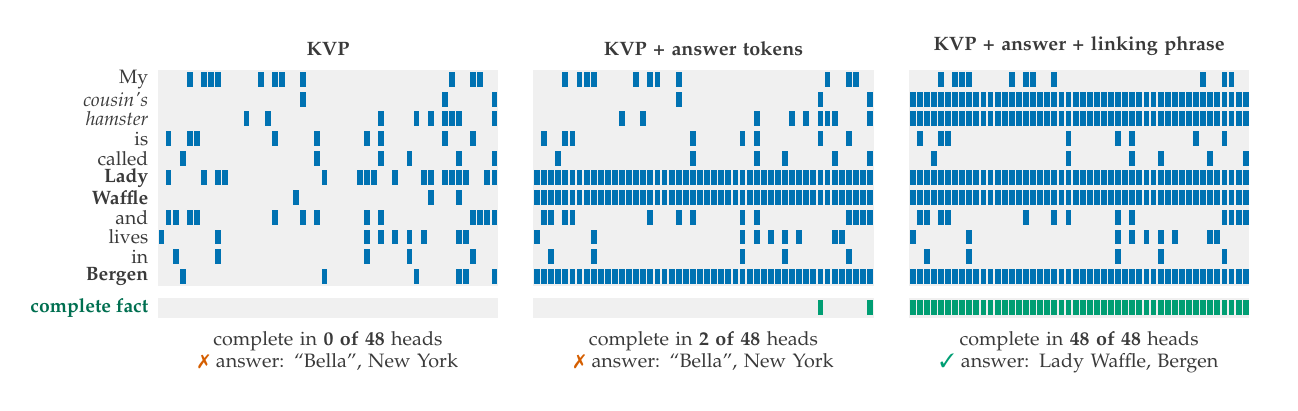
\begin{tikzpicture}[every node/.style={text=cink}]
\node[anchor=east, font=\scriptsize, inner sep=1pt] at (-0.08,-0.125) {My};
\node[anchor=east, font=\scriptsize, inner sep=1pt] at (-0.08,-0.375) {\textit{cousin\textquotesingle{}s}};
\node[anchor=east, font=\scriptsize, inner sep=1pt] at (-0.08,-0.625) {\textit{hamster}};
\node[anchor=east, font=\scriptsize, inner sep=1pt] at (-0.08,-0.875) {is};
\node[anchor=east, font=\scriptsize, inner sep=1pt] at (-0.08,-1.125) {called};
\node[anchor=east, font=\scriptsize, inner sep=1pt] at (-0.08,-1.375) {\textbf{Lady}};
\node[anchor=east, font=\scriptsize, inner sep=1pt] at (-0.08,-1.625) {\textbf{Waffle}};
\node[anchor=east, font=\scriptsize, inner sep=1pt] at (-0.08,-1.875) {and};
\node[anchor=east, font=\scriptsize, inner sep=1pt] at (-0.08,-2.125) {lives};
\node[anchor=east, font=\scriptsize, inner sep=1pt] at (-0.08,-2.375) {in};
\node[anchor=east, font=\scriptsize, inner sep=1pt] at (-0.08,-2.625) {\textbf{Bergen}};
\node[anchor=east, font=\scriptsize\bfseries, inner sep=1pt, text=crest!70!black] at (-0.08,-3.025) {complete fact};
\fill[black!6] (0.000,0) rectangle (4.320,-2.750);
\fill[ckvp] (0.368,-0.030) rectangle (0.442,-0.220);
\fill[ckvp] (0.548,-0.030) rectangle (0.622,-0.220);
\fill[ckvp] (0.638,-0.030) rectangle (0.712,-0.220);
\fill[ckvp] (0.728,-0.030) rectangle (0.802,-0.220);
\fill[ckvp] (1.268,-0.030) rectangle (1.342,-0.220);
\fill[ckvp] (1.448,-0.030) rectangle (1.522,-0.220);
\fill[ckvp] (1.538,-0.030) rectangle (1.612,-0.220);
\fill[ckvp] (1.808,-0.030) rectangle (1.882,-0.220);
\fill[ckvp] (3.698,-0.030) rectangle (3.772,-0.220);
\fill[ckvp] (3.968,-0.030) rectangle (4.042,-0.220);
\fill[ckvp] (4.058,-0.030) rectangle (4.132,-0.220);
\fill[ckvp] (1.808,-0.280) rectangle (1.882,-0.470);
\fill[ckvp] (3.608,-0.280) rectangle (3.682,-0.470);
\fill[ckvp] (4.238,-0.280) rectangle (4.312,-0.470);
\fill[ckvp] (1.088,-0.530) rectangle (1.162,-0.720);
\fill[ckvp] (1.358,-0.530) rectangle (1.432,-0.720);
\fill[ckvp] (2.798,-0.530) rectangle (2.872,-0.720);
\fill[ckvp] (3.248,-0.530) rectangle (3.322,-0.720);
\fill[ckvp] (3.428,-0.530) rectangle (3.502,-0.720);
\fill[ckvp] (3.608,-0.530) rectangle (3.682,-0.720);
\fill[ckvp] (3.698,-0.530) rectangle (3.772,-0.720);
\fill[ckvp] (3.788,-0.530) rectangle (3.862,-0.720);
\fill[ckvp] (4.238,-0.530) rectangle (4.312,-0.720);
\fill[ckvp] (0.098,-0.780) rectangle (0.172,-0.970);
\fill[ckvp] (0.368,-0.780) rectangle (0.442,-0.970);
\fill[ckvp] (0.458,-0.780) rectangle (0.532,-0.970);
\fill[ckvp] (1.448,-0.780) rectangle (1.522,-0.970);
\fill[ckvp] (1.988,-0.780) rectangle (2.062,-0.970);
\fill[ckvp] (2.618,-0.780) rectangle (2.692,-0.970);
\fill[ckvp] (2.798,-0.780) rectangle (2.872,-0.970);
\fill[ckvp] (3.608,-0.780) rectangle (3.682,-0.970);
\fill[ckvp] (3.968,-0.780) rectangle (4.042,-0.970);
\fill[ckvp] (0.278,-1.030) rectangle (0.352,-1.220);
\fill[ckvp] (1.988,-1.030) rectangle (2.062,-1.220);
\fill[ckvp] (2.798,-1.030) rectangle (2.872,-1.220);
\fill[ckvp] (3.158,-1.030) rectangle (3.232,-1.220);
\fill[ckvp] (3.788,-1.030) rectangle (3.862,-1.220);
\fill[ckvp] (4.238,-1.030) rectangle (4.312,-1.220);
\fill[ckvp] (0.098,-1.280) rectangle (0.172,-1.470);
\fill[ckvp] (0.548,-1.280) rectangle (0.622,-1.470);
\fill[ckvp] (0.728,-1.280) rectangle (0.802,-1.470);
\fill[ckvp] (0.818,-1.280) rectangle (0.892,-1.470);
\fill[ckvp] (2.078,-1.280) rectangle (2.152,-1.470);
\fill[ckvp] (2.528,-1.280) rectangle (2.602,-1.470);
\fill[ckvp] (2.618,-1.280) rectangle (2.692,-1.470);
\fill[ckvp] (2.708,-1.280) rectangle (2.782,-1.470);
\fill[ckvp] (2.978,-1.280) rectangle (3.052,-1.470);
\fill[ckvp] (3.338,-1.280) rectangle (3.412,-1.470);
\fill[ckvp] (3.428,-1.280) rectangle (3.502,-1.470);
\fill[ckvp] (3.608,-1.280) rectangle (3.682,-1.470);
\fill[ckvp] (3.698,-1.280) rectangle (3.772,-1.470);
\fill[ckvp] (3.788,-1.280) rectangle (3.862,-1.470);
\fill[ckvp] (3.878,-1.280) rectangle (3.952,-1.470);
\fill[ckvp] (4.148,-1.280) rectangle (4.222,-1.470);
\fill[ckvp] (4.238,-1.280) rectangle (4.312,-1.470);
\fill[ckvp] (1.718,-1.530) rectangle (1.792,-1.720);
\fill[ckvp] (3.428,-1.530) rectangle (3.502,-1.720);
\fill[ckvp] (3.788,-1.530) rectangle (3.862,-1.720);
\fill[ckvp] (0.098,-1.780) rectangle (0.172,-1.970);
\fill[ckvp] (0.188,-1.780) rectangle (0.262,-1.970);
\fill[ckvp] (0.368,-1.780) rectangle (0.442,-1.970);
\fill[ckvp] (0.458,-1.780) rectangle (0.532,-1.970);
\fill[ckvp] (1.448,-1.780) rectangle (1.522,-1.970);
\fill[ckvp] (1.808,-1.780) rectangle (1.882,-1.970);
\fill[ckvp] (1.988,-1.780) rectangle (2.062,-1.970);
\fill[ckvp] (2.618,-1.780) rectangle (2.692,-1.970);
\fill[ckvp] (2.798,-1.780) rectangle (2.872,-1.970);
\fill[ckvp] (3.968,-1.780) rectangle (4.042,-1.970);
\fill[ckvp] (4.058,-1.780) rectangle (4.132,-1.970);
\fill[ckvp] (4.148,-1.780) rectangle (4.222,-1.970);
\fill[ckvp] (4.238,-1.780) rectangle (4.312,-1.970);
\fill[ckvp] (0.008,-2.030) rectangle (0.082,-2.220);
\fill[ckvp] (0.728,-2.030) rectangle (0.802,-2.220);
\fill[ckvp] (2.618,-2.030) rectangle (2.692,-2.220);
\fill[ckvp] (2.798,-2.030) rectangle (2.872,-2.220);
\fill[ckvp] (2.978,-2.030) rectangle (3.052,-2.220);
\fill[ckvp] (3.158,-2.030) rectangle (3.232,-2.220);
\fill[ckvp] (3.338,-2.030) rectangle (3.412,-2.220);
\fill[ckvp] (3.788,-2.030) rectangle (3.862,-2.220);
\fill[ckvp] (3.878,-2.030) rectangle (3.952,-2.220);
\fill[ckvp] (0.188,-2.280) rectangle (0.262,-2.470);
\fill[ckvp] (0.728,-2.280) rectangle (0.802,-2.470);
\fill[ckvp] (2.618,-2.280) rectangle (2.692,-2.470);
\fill[ckvp] (3.158,-2.280) rectangle (3.232,-2.470);
\fill[ckvp] (3.968,-2.280) rectangle (4.042,-2.470);
\fill[ckvp] (0.278,-2.530) rectangle (0.352,-2.720);
\fill[ckvp] (2.078,-2.530) rectangle (2.152,-2.720);
\fill[ckvp] (3.248,-2.530) rectangle (3.322,-2.720);
\fill[ckvp] (3.788,-2.530) rectangle (3.862,-2.720);
\fill[ckvp] (3.878,-2.530) rectangle (3.952,-2.720);
\fill[ckvp] (4.238,-2.530) rectangle (4.312,-2.720);
\fill[black!6] (0.000,-2.900) rectangle (4.320,-3.150);
\node[anchor=south, font=\scriptsize\bfseries, align=center, text width=4.62cm] at (2.160,0.05) {KVP};
\node[anchor=north, font=\scriptsize, align=center, text width=4.62cm] at (2.160,-3.200) {complete in \textbf{0 of 48} heads\\ \xmark\ answer: ``Bella'', New York};
\fill[black!6] (4.770,0) rectangle (9.090,-2.750);
\fill[ckvp] (5.138,-0.030) rectangle (5.212,-0.220);
\fill[ckvp] (5.318,-0.030) rectangle (5.392,-0.220);
\fill[ckvp] (5.408,-0.030) rectangle (5.482,-0.220);
\fill[ckvp] (5.498,-0.030) rectangle (5.572,-0.220);
\fill[ckvp] (6.038,-0.030) rectangle (6.112,-0.220);
\fill[ckvp] (6.218,-0.030) rectangle (6.292,-0.220);
\fill[ckvp] (6.308,-0.030) rectangle (6.382,-0.220);
\fill[ckvp] (6.578,-0.030) rectangle (6.652,-0.220);
\fill[ckvp] (8.468,-0.030) rectangle (8.542,-0.220);
\fill[ckvp] (8.738,-0.030) rectangle (8.812,-0.220);
\fill[ckvp] (8.828,-0.030) rectangle (8.902,-0.220);
\fill[ckvp] (6.578,-0.280) rectangle (6.652,-0.470);
\fill[ckvp] (8.378,-0.280) rectangle (8.452,-0.470);
\fill[ckvp] (9.008,-0.280) rectangle (9.082,-0.470);
\fill[ckvp] (5.858,-0.530) rectangle (5.932,-0.720);
\fill[ckvp] (6.128,-0.530) rectangle (6.202,-0.720);
\fill[ckvp] (7.568,-0.530) rectangle (7.642,-0.720);
\fill[ckvp] (8.018,-0.530) rectangle (8.092,-0.720);
\fill[ckvp] (8.198,-0.530) rectangle (8.272,-0.720);
\fill[ckvp] (8.378,-0.530) rectangle (8.452,-0.720);
\fill[ckvp] (8.468,-0.530) rectangle (8.542,-0.720);
\fill[ckvp] (8.558,-0.530) rectangle (8.632,-0.720);
\fill[ckvp] (9.008,-0.530) rectangle (9.082,-0.720);
\fill[ckvp] (4.868,-0.780) rectangle (4.942,-0.970);
\fill[ckvp] (5.138,-0.780) rectangle (5.212,-0.970);
\fill[ckvp] (5.228,-0.780) rectangle (5.302,-0.970);
\fill[ckvp] (6.758,-0.780) rectangle (6.832,-0.970);
\fill[ckvp] (7.388,-0.780) rectangle (7.462,-0.970);
\fill[ckvp] (7.568,-0.780) rectangle (7.642,-0.970);
\fill[ckvp] (8.378,-0.780) rectangle (8.452,-0.970);
\fill[ckvp] (8.738,-0.780) rectangle (8.812,-0.970);
\fill[ckvp] (5.048,-1.030) rectangle (5.122,-1.220);
\fill[ckvp] (6.758,-1.030) rectangle (6.832,-1.220);
\fill[ckvp] (7.568,-1.030) rectangle (7.642,-1.220);
\fill[ckvp] (7.928,-1.030) rectangle (8.002,-1.220);
\fill[ckvp] (8.558,-1.030) rectangle (8.632,-1.220);
\fill[ckvp] (9.008,-1.030) rectangle (9.082,-1.220);
\fill[ckvp] (4.778,-1.280) rectangle (4.852,-1.470);
\fill[ckvp] (4.868,-1.280) rectangle (4.942,-1.470);
\fill[ckvp] (4.958,-1.280) rectangle (5.032,-1.470);
\fill[ckvp] (5.048,-1.280) rectangle (5.122,-1.470);
\fill[ckvp] (5.138,-1.280) rectangle (5.212,-1.470);
\fill[ckvp] (5.228,-1.280) rectangle (5.302,-1.470);
\fill[ckvp] (5.318,-1.280) rectangle (5.392,-1.470);
\fill[ckvp] (5.408,-1.280) rectangle (5.482,-1.470);
\fill[ckvp] (5.498,-1.280) rectangle (5.572,-1.470);
\fill[ckvp] (5.588,-1.280) rectangle (5.662,-1.470);
\fill[ckvp] (5.678,-1.280) rectangle (5.752,-1.470);
\fill[ckvp] (5.768,-1.280) rectangle (5.842,-1.470);
\fill[ckvp] (5.858,-1.280) rectangle (5.932,-1.470);
\fill[ckvp] (5.948,-1.280) rectangle (6.022,-1.470);
\fill[ckvp] (6.038,-1.280) rectangle (6.112,-1.470);
\fill[ckvp] (6.128,-1.280) rectangle (6.202,-1.470);
\fill[ckvp] (6.218,-1.280) rectangle (6.292,-1.470);
\fill[ckvp] (6.308,-1.280) rectangle (6.382,-1.470);
\fill[ckvp] (6.398,-1.280) rectangle (6.472,-1.470);
\fill[ckvp] (6.488,-1.280) rectangle (6.562,-1.470);
\fill[ckvp] (6.578,-1.280) rectangle (6.652,-1.470);
\fill[ckvp] (6.668,-1.280) rectangle (6.742,-1.470);
\fill[ckvp] (6.758,-1.280) rectangle (6.832,-1.470);
\fill[ckvp] (6.848,-1.280) rectangle (6.922,-1.470);
\fill[ckvp] (6.938,-1.280) rectangle (7.012,-1.470);
\fill[ckvp] (7.028,-1.280) rectangle (7.102,-1.470);
\fill[ckvp] (7.118,-1.280) rectangle (7.192,-1.470);
\fill[ckvp] (7.208,-1.280) rectangle (7.282,-1.470);
\fill[ckvp] (7.298,-1.280) rectangle (7.372,-1.470);
\fill[ckvp] (7.388,-1.280) rectangle (7.462,-1.470);
\fill[ckvp] (7.478,-1.280) rectangle (7.552,-1.470);
\fill[ckvp] (7.568,-1.280) rectangle (7.642,-1.470);
\fill[ckvp] (7.658,-1.280) rectangle (7.732,-1.470);
\fill[ckvp] (7.748,-1.280) rectangle (7.822,-1.470);
\fill[ckvp] (7.838,-1.280) rectangle (7.912,-1.470);
\fill[ckvp] (7.928,-1.280) rectangle (8.002,-1.470);
\fill[ckvp] (8.018,-1.280) rectangle (8.092,-1.470);
\fill[ckvp] (8.108,-1.280) rectangle (8.182,-1.470);
\fill[ckvp] (8.198,-1.280) rectangle (8.272,-1.470);
\fill[ckvp] (8.288,-1.280) rectangle (8.362,-1.470);
\fill[ckvp] (8.378,-1.280) rectangle (8.452,-1.470);
\fill[ckvp] (8.468,-1.280) rectangle (8.542,-1.470);
\fill[ckvp] (8.558,-1.280) rectangle (8.632,-1.470);
\fill[ckvp] (8.648,-1.280) rectangle (8.722,-1.470);
\fill[ckvp] (8.738,-1.280) rectangle (8.812,-1.470);
\fill[ckvp] (8.828,-1.280) rectangle (8.902,-1.470);
\fill[ckvp] (8.918,-1.280) rectangle (8.992,-1.470);
\fill[ckvp] (9.008,-1.280) rectangle (9.082,-1.470);
\fill[ckvp] (4.778,-1.530) rectangle (4.852,-1.720);
\fill[ckvp] (4.868,-1.530) rectangle (4.942,-1.720);
\fill[ckvp] (4.958,-1.530) rectangle (5.032,-1.720);
\fill[ckvp] (5.048,-1.530) rectangle (5.122,-1.720);
\fill[ckvp] (5.138,-1.530) rectangle (5.212,-1.720);
\fill[ckvp] (5.228,-1.530) rectangle (5.302,-1.720);
\fill[ckvp] (5.318,-1.530) rectangle (5.392,-1.720);
\fill[ckvp] (5.408,-1.530) rectangle (5.482,-1.720);
\fill[ckvp] (5.498,-1.530) rectangle (5.572,-1.720);
\fill[ckvp] (5.588,-1.530) rectangle (5.662,-1.720);
\fill[ckvp] (5.678,-1.530) rectangle (5.752,-1.720);
\fill[ckvp] (5.768,-1.530) rectangle (5.842,-1.720);
\fill[ckvp] (5.858,-1.530) rectangle (5.932,-1.720);
\fill[ckvp] (5.948,-1.530) rectangle (6.022,-1.720);
\fill[ckvp] (6.038,-1.530) rectangle (6.112,-1.720);
\fill[ckvp] (6.128,-1.530) rectangle (6.202,-1.720);
\fill[ckvp] (6.218,-1.530) rectangle (6.292,-1.720);
\fill[ckvp] (6.308,-1.530) rectangle (6.382,-1.720);
\fill[ckvp] (6.398,-1.530) rectangle (6.472,-1.720);
\fill[ckvp] (6.488,-1.530) rectangle (6.562,-1.720);
\fill[ckvp] (6.578,-1.530) rectangle (6.652,-1.720);
\fill[ckvp] (6.668,-1.530) rectangle (6.742,-1.720);
\fill[ckvp] (6.758,-1.530) rectangle (6.832,-1.720);
\fill[ckvp] (6.848,-1.530) rectangle (6.922,-1.720);
\fill[ckvp] (6.938,-1.530) rectangle (7.012,-1.720);
\fill[ckvp] (7.028,-1.530) rectangle (7.102,-1.720);
\fill[ckvp] (7.118,-1.530) rectangle (7.192,-1.720);
\fill[ckvp] (7.208,-1.530) rectangle (7.282,-1.720);
\fill[ckvp] (7.298,-1.530) rectangle (7.372,-1.720);
\fill[ckvp] (7.388,-1.530) rectangle (7.462,-1.720);
\fill[ckvp] (7.478,-1.530) rectangle (7.552,-1.720);
\fill[ckvp] (7.568,-1.530) rectangle (7.642,-1.720);
\fill[ckvp] (7.658,-1.530) rectangle (7.732,-1.720);
\fill[ckvp] (7.748,-1.530) rectangle (7.822,-1.720);
\fill[ckvp] (7.838,-1.530) rectangle (7.912,-1.720);
\fill[ckvp] (7.928,-1.530) rectangle (8.002,-1.720);
\fill[ckvp] (8.018,-1.530) rectangle (8.092,-1.720);
\fill[ckvp] (8.108,-1.530) rectangle (8.182,-1.720);
\fill[ckvp] (8.198,-1.530) rectangle (8.272,-1.720);
\fill[ckvp] (8.288,-1.530) rectangle (8.362,-1.720);
\fill[ckvp] (8.378,-1.530) rectangle (8.452,-1.720);
\fill[ckvp] (8.468,-1.530) rectangle (8.542,-1.720);
\fill[ckvp] (8.558,-1.530) rectangle (8.632,-1.720);
\fill[ckvp] (8.648,-1.530) rectangle (8.722,-1.720);
\fill[ckvp] (8.738,-1.530) rectangle (8.812,-1.720);
\fill[ckvp] (8.828,-1.530) rectangle (8.902,-1.720);
\fill[ckvp] (8.918,-1.530) rectangle (8.992,-1.720);
\fill[ckvp] (9.008,-1.530) rectangle (9.082,-1.720);
\fill[ckvp] (4.868,-1.780) rectangle (4.942,-1.970);
\fill[ckvp] (4.958,-1.780) rectangle (5.032,-1.970);
\fill[ckvp] (5.138,-1.780) rectangle (5.212,-1.970);
\fill[ckvp] (5.228,-1.780) rectangle (5.302,-1.970);
\fill[ckvp] (6.218,-1.780) rectangle (6.292,-1.970);
\fill[ckvp] (6.578,-1.780) rectangle (6.652,-1.970);
\fill[ckvp] (6.758,-1.780) rectangle (6.832,-1.970);
\fill[ckvp] (7.388,-1.780) rectangle (7.462,-1.970);
\fill[ckvp] (7.568,-1.780) rectangle (7.642,-1.970);
\fill[ckvp] (8.738,-1.780) rectangle (8.812,-1.970);
\fill[ckvp] (8.828,-1.780) rectangle (8.902,-1.970);
\fill[ckvp] (8.918,-1.780) rectangle (8.992,-1.970);
\fill[ckvp] (9.008,-1.780) rectangle (9.082,-1.970);
\fill[ckvp] (4.778,-2.030) rectangle (4.852,-2.220);
\fill[ckvp] (5.498,-2.030) rectangle (5.572,-2.220);
\fill[ckvp] (7.388,-2.030) rectangle (7.462,-2.220);
\fill[ckvp] (7.568,-2.030) rectangle (7.642,-2.220);
\fill[ckvp] (7.748,-2.030) rectangle (7.822,-2.220);
\fill[ckvp] (7.928,-2.030) rectangle (8.002,-2.220);
\fill[ckvp] (8.108,-2.030) rectangle (8.182,-2.220);
\fill[ckvp] (8.558,-2.030) rectangle (8.632,-2.220);
\fill[ckvp] (8.648,-2.030) rectangle (8.722,-2.220);
\fill[ckvp] (4.958,-2.280) rectangle (5.032,-2.470);
\fill[ckvp] (5.498,-2.280) rectangle (5.572,-2.470);
\fill[ckvp] (7.388,-2.280) rectangle (7.462,-2.470);
\fill[ckvp] (7.928,-2.280) rectangle (8.002,-2.470);
\fill[ckvp] (8.738,-2.280) rectangle (8.812,-2.470);
\fill[ckvp] (4.778,-2.530) rectangle (4.852,-2.720);
\fill[ckvp] (4.868,-2.530) rectangle (4.942,-2.720);
\fill[ckvp] (4.958,-2.530) rectangle (5.032,-2.720);
\fill[ckvp] (5.048,-2.530) rectangle (5.122,-2.720);
\fill[ckvp] (5.138,-2.530) rectangle (5.212,-2.720);
\fill[ckvp] (5.228,-2.530) rectangle (5.302,-2.720);
\fill[ckvp] (5.318,-2.530) rectangle (5.392,-2.720);
\fill[ckvp] (5.408,-2.530) rectangle (5.482,-2.720);
\fill[ckvp] (5.498,-2.530) rectangle (5.572,-2.720);
\fill[ckvp] (5.588,-2.530) rectangle (5.662,-2.720);
\fill[ckvp] (5.678,-2.530) rectangle (5.752,-2.720);
\fill[ckvp] (5.768,-2.530) rectangle (5.842,-2.720);
\fill[ckvp] (5.858,-2.530) rectangle (5.932,-2.720);
\fill[ckvp] (5.948,-2.530) rectangle (6.022,-2.720);
\fill[ckvp] (6.038,-2.530) rectangle (6.112,-2.720);
\fill[ckvp] (6.128,-2.530) rectangle (6.202,-2.720);
\fill[ckvp] (6.218,-2.530) rectangle (6.292,-2.720);
\fill[ckvp] (6.308,-2.530) rectangle (6.382,-2.720);
\fill[ckvp] (6.398,-2.530) rectangle (6.472,-2.720);
\fill[ckvp] (6.488,-2.530) rectangle (6.562,-2.720);
\fill[ckvp] (6.578,-2.530) rectangle (6.652,-2.720);
\fill[ckvp] (6.668,-2.530) rectangle (6.742,-2.720);
\fill[ckvp] (6.758,-2.530) rectangle (6.832,-2.720);
\fill[ckvp] (6.848,-2.530) rectangle (6.922,-2.720);
\fill[ckvp] (6.938,-2.530) rectangle (7.012,-2.720);
\fill[ckvp] (7.028,-2.530) rectangle (7.102,-2.720);
\fill[ckvp] (7.118,-2.530) rectangle (7.192,-2.720);
\fill[ckvp] (7.208,-2.530) rectangle (7.282,-2.720);
\fill[ckvp] (7.298,-2.530) rectangle (7.372,-2.720);
\fill[ckvp] (7.388,-2.530) rectangle (7.462,-2.720);
\fill[ckvp] (7.478,-2.530) rectangle (7.552,-2.720);
\fill[ckvp] (7.568,-2.530) rectangle (7.642,-2.720);
\fill[ckvp] (7.658,-2.530) rectangle (7.732,-2.720);
\fill[ckvp] (7.748,-2.530) rectangle (7.822,-2.720);
\fill[ckvp] (7.838,-2.530) rectangle (7.912,-2.720);
\fill[ckvp] (7.928,-2.530) rectangle (8.002,-2.720);
\fill[ckvp] (8.018,-2.530) rectangle (8.092,-2.720);
\fill[ckvp] (8.108,-2.530) rectangle (8.182,-2.720);
\fill[ckvp] (8.198,-2.530) rectangle (8.272,-2.720);
\fill[ckvp] (8.288,-2.530) rectangle (8.362,-2.720);
\fill[ckvp] (8.378,-2.530) rectangle (8.452,-2.720);
\fill[ckvp] (8.468,-2.530) rectangle (8.542,-2.720);
\fill[ckvp] (8.558,-2.530) rectangle (8.632,-2.720);
\fill[ckvp] (8.648,-2.530) rectangle (8.722,-2.720);
\fill[ckvp] (8.738,-2.530) rectangle (8.812,-2.720);
\fill[ckvp] (8.828,-2.530) rectangle (8.902,-2.720);
\fill[ckvp] (8.918,-2.530) rectangle (8.992,-2.720);
\fill[ckvp] (9.008,-2.530) rectangle (9.082,-2.720);
\fill[black!6] (4.770,-2.900) rectangle (9.090,-3.150);
\fill[crest] (8.378,-2.930) rectangle (8.452,-3.120);
\fill[crest] (9.008,-2.930) rectangle (9.082,-3.120);
\node[anchor=south, font=\scriptsize\bfseries, align=center, text width=4.62cm] at (6.930,0.05) {KVP + answer tokens};
\node[anchor=north, font=\scriptsize, align=center, text width=4.62cm] at (6.930,-3.200) {complete in \textbf{2 of 48} heads\\ \xmark\ answer: ``Bella'', New York};
\fill[black!6] (9.540,0) rectangle (13.860,-2.750);
\fill[ckvp] (9.908,-0.030) rectangle (9.982,-0.220);
\fill[ckvp] (10.088,-0.030) rectangle (10.162,-0.220);
\fill[ckvp] (10.178,-0.030) rectangle (10.252,-0.220);
\fill[ckvp] (10.268,-0.030) rectangle (10.342,-0.220);
\fill[ckvp] (10.808,-0.030) rectangle (10.882,-0.220);
\fill[ckvp] (10.988,-0.030) rectangle (11.062,-0.220);
\fill[ckvp] (11.078,-0.030) rectangle (11.152,-0.220);
\fill[ckvp] (11.348,-0.030) rectangle (11.422,-0.220);
\fill[ckvp] (13.238,-0.030) rectangle (13.312,-0.220);
\fill[ckvp] (13.508,-0.030) rectangle (13.582,-0.220);
\fill[ckvp] (13.598,-0.030) rectangle (13.672,-0.220);
\fill[ckvp] (9.548,-0.280) rectangle (9.622,-0.470);
\fill[ckvp] (9.638,-0.280) rectangle (9.712,-0.470);
\fill[ckvp] (9.728,-0.280) rectangle (9.802,-0.470);
\fill[ckvp] (9.818,-0.280) rectangle (9.892,-0.470);
\fill[ckvp] (9.908,-0.280) rectangle (9.982,-0.470);
\fill[ckvp] (9.998,-0.280) rectangle (10.072,-0.470);
\fill[ckvp] (10.088,-0.280) rectangle (10.162,-0.470);
\fill[ckvp] (10.178,-0.280) rectangle (10.252,-0.470);
\fill[ckvp] (10.268,-0.280) rectangle (10.342,-0.470);
\fill[ckvp] (10.358,-0.280) rectangle (10.432,-0.470);
\fill[ckvp] (10.448,-0.280) rectangle (10.522,-0.470);
\fill[ckvp] (10.538,-0.280) rectangle (10.612,-0.470);
\fill[ckvp] (10.628,-0.280) rectangle (10.702,-0.470);
\fill[ckvp] (10.718,-0.280) rectangle (10.792,-0.470);
\fill[ckvp] (10.808,-0.280) rectangle (10.882,-0.470);
\fill[ckvp] (10.898,-0.280) rectangle (10.972,-0.470);
\fill[ckvp] (10.988,-0.280) rectangle (11.062,-0.470);
\fill[ckvp] (11.078,-0.280) rectangle (11.152,-0.470);
\fill[ckvp] (11.168,-0.280) rectangle (11.242,-0.470);
\fill[ckvp] (11.258,-0.280) rectangle (11.332,-0.470);
\fill[ckvp] (11.348,-0.280) rectangle (11.422,-0.470);
\fill[ckvp] (11.438,-0.280) rectangle (11.512,-0.470);
\fill[ckvp] (11.528,-0.280) rectangle (11.602,-0.470);
\fill[ckvp] (11.618,-0.280) rectangle (11.692,-0.470);
\fill[ckvp] (11.708,-0.280) rectangle (11.782,-0.470);
\fill[ckvp] (11.798,-0.280) rectangle (11.872,-0.470);
\fill[ckvp] (11.888,-0.280) rectangle (11.962,-0.470);
\fill[ckvp] (11.978,-0.280) rectangle (12.052,-0.470);
\fill[ckvp] (12.068,-0.280) rectangle (12.142,-0.470);
\fill[ckvp] (12.158,-0.280) rectangle (12.232,-0.470);
\fill[ckvp] (12.248,-0.280) rectangle (12.322,-0.470);
\fill[ckvp] (12.338,-0.280) rectangle (12.412,-0.470);
\fill[ckvp] (12.428,-0.280) rectangle (12.502,-0.470);
\fill[ckvp] (12.518,-0.280) rectangle (12.592,-0.470);
\fill[ckvp] (12.608,-0.280) rectangle (12.682,-0.470);
\fill[ckvp] (12.698,-0.280) rectangle (12.772,-0.470);
\fill[ckvp] (12.788,-0.280) rectangle (12.862,-0.470);
\fill[ckvp] (12.878,-0.280) rectangle (12.952,-0.470);
\fill[ckvp] (12.968,-0.280) rectangle (13.042,-0.470);
\fill[ckvp] (13.058,-0.280) rectangle (13.132,-0.470);
\fill[ckvp] (13.148,-0.280) rectangle (13.222,-0.470);
\fill[ckvp] (13.238,-0.280) rectangle (13.312,-0.470);
\fill[ckvp] (13.328,-0.280) rectangle (13.402,-0.470);
\fill[ckvp] (13.418,-0.280) rectangle (13.492,-0.470);
\fill[ckvp] (13.508,-0.280) rectangle (13.582,-0.470);
\fill[ckvp] (13.598,-0.280) rectangle (13.672,-0.470);
\fill[ckvp] (13.688,-0.280) rectangle (13.762,-0.470);
\fill[ckvp] (13.778,-0.280) rectangle (13.852,-0.470);
\fill[ckvp] (9.548,-0.530) rectangle (9.622,-0.720);
\fill[ckvp] (9.638,-0.530) rectangle (9.712,-0.720);
\fill[ckvp] (9.728,-0.530) rectangle (9.802,-0.720);
\fill[ckvp] (9.818,-0.530) rectangle (9.892,-0.720);
\fill[ckvp] (9.908,-0.530) rectangle (9.982,-0.720);
\fill[ckvp] (9.998,-0.530) rectangle (10.072,-0.720);
\fill[ckvp] (10.088,-0.530) rectangle (10.162,-0.720);
\fill[ckvp] (10.178,-0.530) rectangle (10.252,-0.720);
\fill[ckvp] (10.268,-0.530) rectangle (10.342,-0.720);
\fill[ckvp] (10.358,-0.530) rectangle (10.432,-0.720);
\fill[ckvp] (10.448,-0.530) rectangle (10.522,-0.720);
\fill[ckvp] (10.538,-0.530) rectangle (10.612,-0.720);
\fill[ckvp] (10.628,-0.530) rectangle (10.702,-0.720);
\fill[ckvp] (10.718,-0.530) rectangle (10.792,-0.720);
\fill[ckvp] (10.808,-0.530) rectangle (10.882,-0.720);
\fill[ckvp] (10.898,-0.530) rectangle (10.972,-0.720);
\fill[ckvp] (10.988,-0.530) rectangle (11.062,-0.720);
\fill[ckvp] (11.078,-0.530) rectangle (11.152,-0.720);
\fill[ckvp] (11.168,-0.530) rectangle (11.242,-0.720);
\fill[ckvp] (11.258,-0.530) rectangle (11.332,-0.720);
\fill[ckvp] (11.348,-0.530) rectangle (11.422,-0.720);
\fill[ckvp] (11.438,-0.530) rectangle (11.512,-0.720);
\fill[ckvp] (11.528,-0.530) rectangle (11.602,-0.720);
\fill[ckvp] (11.618,-0.530) rectangle (11.692,-0.720);
\fill[ckvp] (11.708,-0.530) rectangle (11.782,-0.720);
\fill[ckvp] (11.798,-0.530) rectangle (11.872,-0.720);
\fill[ckvp] (11.888,-0.530) rectangle (11.962,-0.720);
\fill[ckvp] (11.978,-0.530) rectangle (12.052,-0.720);
\fill[ckvp] (12.068,-0.530) rectangle (12.142,-0.720);
\fill[ckvp] (12.158,-0.530) rectangle (12.232,-0.720);
\fill[ckvp] (12.248,-0.530) rectangle (12.322,-0.720);
\fill[ckvp] (12.338,-0.530) rectangle (12.412,-0.720);
\fill[ckvp] (12.428,-0.530) rectangle (12.502,-0.720);
\fill[ckvp] (12.518,-0.530) rectangle (12.592,-0.720);
\fill[ckvp] (12.608,-0.530) rectangle (12.682,-0.720);
\fill[ckvp] (12.698,-0.530) rectangle (12.772,-0.720);
\fill[ckvp] (12.788,-0.530) rectangle (12.862,-0.720);
\fill[ckvp] (12.878,-0.530) rectangle (12.952,-0.720);
\fill[ckvp] (12.968,-0.530) rectangle (13.042,-0.720);
\fill[ckvp] (13.058,-0.530) rectangle (13.132,-0.720);
\fill[ckvp] (13.148,-0.530) rectangle (13.222,-0.720);
\fill[ckvp] (13.238,-0.530) rectangle (13.312,-0.720);
\fill[ckvp] (13.328,-0.530) rectangle (13.402,-0.720);
\fill[ckvp] (13.418,-0.530) rectangle (13.492,-0.720);
\fill[ckvp] (13.508,-0.530) rectangle (13.582,-0.720);
\fill[ckvp] (13.598,-0.530) rectangle (13.672,-0.720);
\fill[ckvp] (13.688,-0.530) rectangle (13.762,-0.720);
\fill[ckvp] (13.778,-0.530) rectangle (13.852,-0.720);
\fill[ckvp] (9.638,-0.780) rectangle (9.712,-0.970);
\fill[ckvp] (9.908,-0.780) rectangle (9.982,-0.970);
\fill[ckvp] (9.998,-0.780) rectangle (10.072,-0.970);
\fill[ckvp] (11.528,-0.780) rectangle (11.602,-0.970);
\fill[ckvp] (12.158,-0.780) rectangle (12.232,-0.970);
\fill[ckvp] (12.338,-0.780) rectangle (12.412,-0.970);
\fill[ckvp] (13.148,-0.780) rectangle (13.222,-0.970);
\fill[ckvp] (13.508,-0.780) rectangle (13.582,-0.970);
\fill[ckvp] (9.818,-1.030) rectangle (9.892,-1.220);
\fill[ckvp] (11.528,-1.030) rectangle (11.602,-1.220);
\fill[ckvp] (12.338,-1.030) rectangle (12.412,-1.220);
\fill[ckvp] (12.698,-1.030) rectangle (12.772,-1.220);
\fill[ckvp] (13.328,-1.030) rectangle (13.402,-1.220);
\fill[ckvp] (13.778,-1.030) rectangle (13.852,-1.220);
\fill[ckvp] (9.548,-1.280) rectangle (9.622,-1.470);
\fill[ckvp] (9.638,-1.280) rectangle (9.712,-1.470);
\fill[ckvp] (9.728,-1.280) rectangle (9.802,-1.470);
\fill[ckvp] (9.818,-1.280) rectangle (9.892,-1.470);
\fill[ckvp] (9.908,-1.280) rectangle (9.982,-1.470);
\fill[ckvp] (9.998,-1.280) rectangle (10.072,-1.470);
\fill[ckvp] (10.088,-1.280) rectangle (10.162,-1.470);
\fill[ckvp] (10.178,-1.280) rectangle (10.252,-1.470);
\fill[ckvp] (10.268,-1.280) rectangle (10.342,-1.470);
\fill[ckvp] (10.358,-1.280) rectangle (10.432,-1.470);
\fill[ckvp] (10.448,-1.280) rectangle (10.522,-1.470);
\fill[ckvp] (10.538,-1.280) rectangle (10.612,-1.470);
\fill[ckvp] (10.628,-1.280) rectangle (10.702,-1.470);
\fill[ckvp] (10.718,-1.280) rectangle (10.792,-1.470);
\fill[ckvp] (10.808,-1.280) rectangle (10.882,-1.470);
\fill[ckvp] (10.898,-1.280) rectangle (10.972,-1.470);
\fill[ckvp] (10.988,-1.280) rectangle (11.062,-1.470);
\fill[ckvp] (11.078,-1.280) rectangle (11.152,-1.470);
\fill[ckvp] (11.168,-1.280) rectangle (11.242,-1.470);
\fill[ckvp] (11.258,-1.280) rectangle (11.332,-1.470);
\fill[ckvp] (11.348,-1.280) rectangle (11.422,-1.470);
\fill[ckvp] (11.438,-1.280) rectangle (11.512,-1.470);
\fill[ckvp] (11.528,-1.280) rectangle (11.602,-1.470);
\fill[ckvp] (11.618,-1.280) rectangle (11.692,-1.470);
\fill[ckvp] (11.708,-1.280) rectangle (11.782,-1.470);
\fill[ckvp] (11.798,-1.280) rectangle (11.872,-1.470);
\fill[ckvp] (11.888,-1.280) rectangle (11.962,-1.470);
\fill[ckvp] (11.978,-1.280) rectangle (12.052,-1.470);
\fill[ckvp] (12.068,-1.280) rectangle (12.142,-1.470);
\fill[ckvp] (12.158,-1.280) rectangle (12.232,-1.470);
\fill[ckvp] (12.248,-1.280) rectangle (12.322,-1.470);
\fill[ckvp] (12.338,-1.280) rectangle (12.412,-1.470);
\fill[ckvp] (12.428,-1.280) rectangle (12.502,-1.470);
\fill[ckvp] (12.518,-1.280) rectangle (12.592,-1.470);
\fill[ckvp] (12.608,-1.280) rectangle (12.682,-1.470);
\fill[ckvp] (12.698,-1.280) rectangle (12.772,-1.470);
\fill[ckvp] (12.788,-1.280) rectangle (12.862,-1.470);
\fill[ckvp] (12.878,-1.280) rectangle (12.952,-1.470);
\fill[ckvp] (12.968,-1.280) rectangle (13.042,-1.470);
\fill[ckvp] (13.058,-1.280) rectangle (13.132,-1.470);
\fill[ckvp] (13.148,-1.280) rectangle (13.222,-1.470);
\fill[ckvp] (13.238,-1.280) rectangle (13.312,-1.470);
\fill[ckvp] (13.328,-1.280) rectangle (13.402,-1.470);
\fill[ckvp] (13.418,-1.280) rectangle (13.492,-1.470);
\fill[ckvp] (13.508,-1.280) rectangle (13.582,-1.470);
\fill[ckvp] (13.598,-1.280) rectangle (13.672,-1.470);
\fill[ckvp] (13.688,-1.280) rectangle (13.762,-1.470);
\fill[ckvp] (13.778,-1.280) rectangle (13.852,-1.470);
\fill[ckvp] (9.548,-1.530) rectangle (9.622,-1.720);
\fill[ckvp] (9.638,-1.530) rectangle (9.712,-1.720);
\fill[ckvp] (9.728,-1.530) rectangle (9.802,-1.720);
\fill[ckvp] (9.818,-1.530) rectangle (9.892,-1.720);
\fill[ckvp] (9.908,-1.530) rectangle (9.982,-1.720);
\fill[ckvp] (9.998,-1.530) rectangle (10.072,-1.720);
\fill[ckvp] (10.088,-1.530) rectangle (10.162,-1.720);
\fill[ckvp] (10.178,-1.530) rectangle (10.252,-1.720);
\fill[ckvp] (10.268,-1.530) rectangle (10.342,-1.720);
\fill[ckvp] (10.358,-1.530) rectangle (10.432,-1.720);
\fill[ckvp] (10.448,-1.530) rectangle (10.522,-1.720);
\fill[ckvp] (10.538,-1.530) rectangle (10.612,-1.720);
\fill[ckvp] (10.628,-1.530) rectangle (10.702,-1.720);
\fill[ckvp] (10.718,-1.530) rectangle (10.792,-1.720);
\fill[ckvp] (10.808,-1.530) rectangle (10.882,-1.720);
\fill[ckvp] (10.898,-1.530) rectangle (10.972,-1.720);
\fill[ckvp] (10.988,-1.530) rectangle (11.062,-1.720);
\fill[ckvp] (11.078,-1.530) rectangle (11.152,-1.720);
\fill[ckvp] (11.168,-1.530) rectangle (11.242,-1.720);
\fill[ckvp] (11.258,-1.530) rectangle (11.332,-1.720);
\fill[ckvp] (11.348,-1.530) rectangle (11.422,-1.720);
\fill[ckvp] (11.438,-1.530) rectangle (11.512,-1.720);
\fill[ckvp] (11.528,-1.530) rectangle (11.602,-1.720);
\fill[ckvp] (11.618,-1.530) rectangle (11.692,-1.720);
\fill[ckvp] (11.708,-1.530) rectangle (11.782,-1.720);
\fill[ckvp] (11.798,-1.530) rectangle (11.872,-1.720);
\fill[ckvp] (11.888,-1.530) rectangle (11.962,-1.720);
\fill[ckvp] (11.978,-1.530) rectangle (12.052,-1.720);
\fill[ckvp] (12.068,-1.530) rectangle (12.142,-1.720);
\fill[ckvp] (12.158,-1.530) rectangle (12.232,-1.720);
\fill[ckvp] (12.248,-1.530) rectangle (12.322,-1.720);
\fill[ckvp] (12.338,-1.530) rectangle (12.412,-1.720);
\fill[ckvp] (12.428,-1.530) rectangle (12.502,-1.720);
\fill[ckvp] (12.518,-1.530) rectangle (12.592,-1.720);
\fill[ckvp] (12.608,-1.530) rectangle (12.682,-1.720);
\fill[ckvp] (12.698,-1.530) rectangle (12.772,-1.720);
\fill[ckvp] (12.788,-1.530) rectangle (12.862,-1.720);
\fill[ckvp] (12.878,-1.530) rectangle (12.952,-1.720);
\fill[ckvp] (12.968,-1.530) rectangle (13.042,-1.720);
\fill[ckvp] (13.058,-1.530) rectangle (13.132,-1.720);
\fill[ckvp] (13.148,-1.530) rectangle (13.222,-1.720);
\fill[ckvp] (13.238,-1.530) rectangle (13.312,-1.720);
\fill[ckvp] (13.328,-1.530) rectangle (13.402,-1.720);
\fill[ckvp] (13.418,-1.530) rectangle (13.492,-1.720);
\fill[ckvp] (13.508,-1.530) rectangle (13.582,-1.720);
\fill[ckvp] (13.598,-1.530) rectangle (13.672,-1.720);
\fill[ckvp] (13.688,-1.530) rectangle (13.762,-1.720);
\fill[ckvp] (13.778,-1.530) rectangle (13.852,-1.720);
\fill[ckvp] (9.638,-1.780) rectangle (9.712,-1.970);
\fill[ckvp] (9.728,-1.780) rectangle (9.802,-1.970);
\fill[ckvp] (9.908,-1.780) rectangle (9.982,-1.970);
\fill[ckvp] (9.998,-1.780) rectangle (10.072,-1.970);
\fill[ckvp] (10.988,-1.780) rectangle (11.062,-1.970);
\fill[ckvp] (11.348,-1.780) rectangle (11.422,-1.970);
\fill[ckvp] (11.528,-1.780) rectangle (11.602,-1.970);
\fill[ckvp] (12.158,-1.780) rectangle (12.232,-1.970);
\fill[ckvp] (12.338,-1.780) rectangle (12.412,-1.970);
\fill[ckvp] (13.508,-1.780) rectangle (13.582,-1.970);
\fill[ckvp] (13.598,-1.780) rectangle (13.672,-1.970);
\fill[ckvp] (13.688,-1.780) rectangle (13.762,-1.970);
\fill[ckvp] (13.778,-1.780) rectangle (13.852,-1.970);
\fill[ckvp] (9.548,-2.030) rectangle (9.622,-2.220);
\fill[ckvp] (10.268,-2.030) rectangle (10.342,-2.220);
\fill[ckvp] (12.158,-2.030) rectangle (12.232,-2.220);
\fill[ckvp] (12.338,-2.030) rectangle (12.412,-2.220);
\fill[ckvp] (12.518,-2.030) rectangle (12.592,-2.220);
\fill[ckvp] (12.698,-2.030) rectangle (12.772,-2.220);
\fill[ckvp] (12.878,-2.030) rectangle (12.952,-2.220);
\fill[ckvp] (13.328,-2.030) rectangle (13.402,-2.220);
\fill[ckvp] (13.418,-2.030) rectangle (13.492,-2.220);
\fill[ckvp] (9.728,-2.280) rectangle (9.802,-2.470);
\fill[ckvp] (10.268,-2.280) rectangle (10.342,-2.470);
\fill[ckvp] (12.158,-2.280) rectangle (12.232,-2.470);
\fill[ckvp] (12.698,-2.280) rectangle (12.772,-2.470);
\fill[ckvp] (13.508,-2.280) rectangle (13.582,-2.470);
\fill[ckvp] (9.548,-2.530) rectangle (9.622,-2.720);
\fill[ckvp] (9.638,-2.530) rectangle (9.712,-2.720);
\fill[ckvp] (9.728,-2.530) rectangle (9.802,-2.720);
\fill[ckvp] (9.818,-2.530) rectangle (9.892,-2.720);
\fill[ckvp] (9.908,-2.530) rectangle (9.982,-2.720);
\fill[ckvp] (9.998,-2.530) rectangle (10.072,-2.720);
\fill[ckvp] (10.088,-2.530) rectangle (10.162,-2.720);
\fill[ckvp] (10.178,-2.530) rectangle (10.252,-2.720);
\fill[ckvp] (10.268,-2.530) rectangle (10.342,-2.720);
\fill[ckvp] (10.358,-2.530) rectangle (10.432,-2.720);
\fill[ckvp] (10.448,-2.530) rectangle (10.522,-2.720);
\fill[ckvp] (10.538,-2.530) rectangle (10.612,-2.720);
\fill[ckvp] (10.628,-2.530) rectangle (10.702,-2.720);
\fill[ckvp] (10.718,-2.530) rectangle (10.792,-2.720);
\fill[ckvp] (10.808,-2.530) rectangle (10.882,-2.720);
\fill[ckvp] (10.898,-2.530) rectangle (10.972,-2.720);
\fill[ckvp] (10.988,-2.530) rectangle (11.062,-2.720);
\fill[ckvp] (11.078,-2.530) rectangle (11.152,-2.720);
\fill[ckvp] (11.168,-2.530) rectangle (11.242,-2.720);
\fill[ckvp] (11.258,-2.530) rectangle (11.332,-2.720);
\fill[ckvp] (11.348,-2.530) rectangle (11.422,-2.720);
\fill[ckvp] (11.438,-2.530) rectangle (11.512,-2.720);
\fill[ckvp] (11.528,-2.530) rectangle (11.602,-2.720);
\fill[ckvp] (11.618,-2.530) rectangle (11.692,-2.720);
\fill[ckvp] (11.708,-2.530) rectangle (11.782,-2.720);
\fill[ckvp] (11.798,-2.530) rectangle (11.872,-2.720);
\fill[ckvp] (11.888,-2.530) rectangle (11.962,-2.720);
\fill[ckvp] (11.978,-2.530) rectangle (12.052,-2.720);
\fill[ckvp] (12.068,-2.530) rectangle (12.142,-2.720);
\fill[ckvp] (12.158,-2.530) rectangle (12.232,-2.720);
\fill[ckvp] (12.248,-2.530) rectangle (12.322,-2.720);
\fill[ckvp] (12.338,-2.530) rectangle (12.412,-2.720);
\fill[ckvp] (12.428,-2.530) rectangle (12.502,-2.720);
\fill[ckvp] (12.518,-2.530) rectangle (12.592,-2.720);
\fill[ckvp] (12.608,-2.530) rectangle (12.682,-2.720);
\fill[ckvp] (12.698,-2.530) rectangle (12.772,-2.720);
\fill[ckvp] (12.788,-2.530) rectangle (12.862,-2.720);
\fill[ckvp] (12.878,-2.530) rectangle (12.952,-2.720);
\fill[ckvp] (12.968,-2.530) rectangle (13.042,-2.720);
\fill[ckvp] (13.058,-2.530) rectangle (13.132,-2.720);
\fill[ckvp] (13.148,-2.530) rectangle (13.222,-2.720);
\fill[ckvp] (13.238,-2.530) rectangle (13.312,-2.720);
\fill[ckvp] (13.328,-2.530) rectangle (13.402,-2.720);
\fill[ckvp] (13.418,-2.530) rectangle (13.492,-2.720);
\fill[ckvp] (13.508,-2.530) rectangle (13.582,-2.720);
\fill[ckvp] (13.598,-2.530) rectangle (13.672,-2.720);
\fill[ckvp] (13.688,-2.530) rectangle (13.762,-2.720);
\fill[ckvp] (13.778,-2.530) rectangle (13.852,-2.720);
\fill[black!6] (9.540,-2.900) rectangle (13.860,-3.150);
\fill[crest] (9.548,-2.930) rectangle (9.622,-3.120);
\fill[crest] (9.638,-2.930) rectangle (9.712,-3.120);
\fill[crest] (9.728,-2.930) rectangle (9.802,-3.120);
\fill[crest] (9.818,-2.930) rectangle (9.892,-3.120);
\fill[crest] (9.908,-2.930) rectangle (9.982,-3.120);
\fill[crest] (9.998,-2.930) rectangle (10.072,-3.120);
\fill[crest] (10.088,-2.930) rectangle (10.162,-3.120);
\fill[crest] (10.178,-2.930) rectangle (10.252,-3.120);
\fill[crest] (10.268,-2.930) rectangle (10.342,-3.120);
\fill[crest] (10.358,-2.930) rectangle (10.432,-3.120);
\fill[crest] (10.448,-2.930) rectangle (10.522,-3.120);
\fill[crest] (10.538,-2.930) rectangle (10.612,-3.120);
\fill[crest] (10.628,-2.930) rectangle (10.702,-3.120);
\fill[crest] (10.718,-2.930) rectangle (10.792,-3.120);
\fill[crest] (10.808,-2.930) rectangle (10.882,-3.120);
\fill[crest] (10.898,-2.930) rectangle (10.972,-3.120);
\fill[crest] (10.988,-2.930) rectangle (11.062,-3.120);
\fill[crest] (11.078,-2.930) rectangle (11.152,-3.120);
\fill[crest] (11.168,-2.930) rectangle (11.242,-3.120);
\fill[crest] (11.258,-2.930) rectangle (11.332,-3.120);
\fill[crest] (11.348,-2.930) rectangle (11.422,-3.120);
\fill[crest] (11.438,-2.930) rectangle (11.512,-3.120);
\fill[crest] (11.528,-2.930) rectangle (11.602,-3.120);
\fill[crest] (11.618,-2.930) rectangle (11.692,-3.120);
\fill[crest] (11.708,-2.930) rectangle (11.782,-3.120);
\fill[crest] (11.798,-2.930) rectangle (11.872,-3.120);
\fill[crest] (11.888,-2.930) rectangle (11.962,-3.120);
\fill[crest] (11.978,-2.930) rectangle (12.052,-3.120);
\fill[crest] (12.068,-2.930) rectangle (12.142,-3.120);
\fill[crest] (12.158,-2.930) rectangle (12.232,-3.120);
\fill[crest] (12.248,-2.930) rectangle (12.322,-3.120);
\fill[crest] (12.338,-2.930) rectangle (12.412,-3.120);
\fill[crest] (12.428,-2.930) rectangle (12.502,-3.120);
\fill[crest] (12.518,-2.930) rectangle (12.592,-3.120);
\fill[crest] (12.608,-2.930) rectangle (12.682,-3.120);
\fill[crest] (12.698,-2.930) rectangle (12.772,-3.120);
\fill[crest] (12.788,-2.930) rectangle (12.862,-3.120);
\fill[crest] (12.878,-2.930) rectangle (12.952,-3.120);
\fill[crest] (12.968,-2.930) rectangle (13.042,-3.120);
\fill[crest] (13.058,-2.930) rectangle (13.132,-3.120);
\fill[crest] (13.148,-2.930) rectangle (13.222,-3.120);
\fill[crest] (13.238,-2.930) rectangle (13.312,-3.120);
\fill[crest] (13.328,-2.930) rectangle (13.402,-3.120);
\fill[crest] (13.418,-2.930) rectangle (13.492,-3.120);
\fill[crest] (13.508,-2.930) rectangle (13.582,-3.120);
\fill[crest] (13.598,-2.930) rectangle (13.672,-3.120);
\fill[crest] (13.688,-2.930) rectangle (13.762,-3.120);
\fill[crest] (13.778,-2.930) rectangle (13.852,-3.120);
\node[anchor=south, font=\scriptsize\bfseries, align=center, text width=4.62cm] at (11.700,0.05) {KVP + answer + linking phrase};
\node[anchor=north, font=\scriptsize, align=center, text width=4.62cm] at (11.700,-3.200) {complete in \textbf{48 of 48} heads\\ \cmark\ answer: Lady Waffle, Bergen};
\end{tikzpicture}

\caption{Where does each of the 48 KV heads keep the fact when the question arrives? Same dialogue as Fig.~\ref{fig:concept}. Rows: words of the fact sentence (bold: answer; italic: linking phrase); columns: the 48 heads, layer 0 on the left. Blue: the head still holds the word. Green: the head holds the complete fact, linking phrase and answer together. In the second and third panels those words are force-kept in all heads. Layout after \cite{kvp}, Fig.~11.}
\label{fig:heads}
\end{figure}

\section{Setup}

\textbf{Models.} Qwen2.5-0.5B-Instruct (48 KV heads) and Qwen2.5-1.5B-Instruct (56 KV heads) \cite{qwen25}. Apple's KVP weights are not released, so we trained the 48 agents for 0.5B with Apple's code (commit \texttt{d33c2dc}) and the base model frozen: 4,000 steps each on 400 OASST2 \cite{oasst} training traces (of 500; 50 validation, 50 held out), then a 1,500-step warm start on those 400 plus 500 synthetic recall training traces (of 600; 50/50 validation/held out), keeping the checkpoint with the best validation reward. The reward scores how well an agent ranks tokens by future attention in recorded traces, not answer correctness under repeated eviction. On held-out OASST2 traces the agents rank tokens better than StreamingLLM on 41 of 48 heads, but better than an accumulated-attention (H2O-style) ranking on only 28 of 48 (mean cost 1.876 vs 1.895). Apple trained each agent for the same 4,000 steps but on about 4,500 OASST2 samples \cite{kvp}; how our agents compare with theirs is unverified. An OASST2-only control for the extra fine-tuning was not completed (compute ran out), so any change after fine-tuning cannot be attributed to the recall data rather than to extra training. \emph{All KVP results below use these fine-tuned agents}; in an earlier bf16 run the agents before fine-tuning did no better on words (0/119 vs 2/119 at $k = 4, 8$). There are no KVP agents for 1.5B, so tests at that size use StreamingLLM as the base.

\textbf{Eviction.} Evicted keys and values are deleted. After each user message and each reply, every KV head is cut to 256 tokens; the first 4 and last 16 are always kept. Between cuts the cache grows by the new turn. Baselines: full cache, StreamingLLM \cite{streamingllm} (first and most recent tokens) and H2O \cite{h2o} (highest accumulated attention, with the same first/last protection). All methods get the same user messages but write their own replies. Greedy decoding, fp32, one NVIDIA T4.

\textbf{Task.} Each synthetic dialogue has two unrelated OASST2 user turns, the fact as turn 3, $k \in \{4, 8\}$ more unrelated turns, then the question; the model replies to every turn (about 1,000 tokens per dialogue). \emph{Word} facts name an invented pet and its city (correct if the answer contains both and no other listed city); \emph{digit} facts give a five-digit code (correct if the extracted code matches). Each set has 120 dialogues. To locate what must survive, we force the answer tokens, the answer plus the linking phrase (``cousin's hamster''), or the whole user turn (including chat-template tokens) to stay in all heads or in $n$ random heads.

\textbf{Statistics.} Experiments ran in batches with decision rules fixed before each batch; later hypotheses followed earlier results. On the word sets the pre-set full-cache accuracy check failed twice, so every word-set comparison was instead conditioned on full-cache-correct dialogues; this was decided before any eviction method was run on a word set. Accuracy is counted on dialogues the full cache answers: 112/120 (words), 120/120 (digits), 117/120 (words, 1.5B). Methods are compared on the same dialogues with exact McNemar tests (Holm-adjusted within a batch), reported as discordant counts, with Wilson 95\% intervals.

\section{Results}

\subsection{Our KVP agents forget}\label{sec:forgets}
KVP answers 4/112 word facts (3.6\%, CI 1.4--8.8) and 5/120 digit facts (4.2\%, CI 1.8--9.4) (Table~\ref{tab:all}). H2O does better on both, 59/112 and 15/120 (56 vs 1 discordant, $\ph = 1.6\times10^{-15}$; 12 vs 2, $\ph = 0.026$): a simple heuristic beats our learned agents here. Whether better-trained agents would close this gap is open (\S2).

\subsection{What must survive}\label{sec:survive}
Fig.~\ref{fig:heads} shows one dialogue: the complete fact is in 0, 2 and 48 of the 48 heads under KVP, KVP + answer tokens and KVP + answer + linking phrase, and only the last answers correctly. Over the word set, keeping the answer tokens in all heads gives 35/112 under KVP and 0/112 and 0/117 under StreamingLLM at 0.5B and 1.5B (Table~\ref{tab:all}). Adding the linking phrase raises this to 88/112, 105/112 and 116/117 (KVP: 55 vs 2 discordant, $\ph = 4.6\times10^{-14}$; 1.5B: 116 vs 0, $\ph = 7.2\times10^{-35}$); the whole user turn gives 112/112, 112/112 and 116/117. Under KVP, answer + linking phrase is weaker at the longer gap ($k = 4$: 55/58; $k = 8$: 33/54). The pattern holds at both sizes and supports a role for the linking phrase, but adding it also retains more tokens (3--4 per dialogue): equal-size controls (unrelated tokens, a wrong-subject phrase) are not yet run. On digits, answer-only protection achieves 111/120.

\begin{table}[t]
\centering\footnotesize
\caption{Recall (correct/dialogues; $k = 4, 8$; 256 retained tokens per KV head), counted only on dialogues the full cache answers (112/120, 120/120, 117/120), so full cache is 100\% by construction. Bold: best usable method per column. Diagnostic rows force part of the fact to stay in the cache (all heads unless stated), which needs its position: a probe, not a method. ``Whole user turn'' includes chat-template tokens. Restore uses an extra CPU archive. --: not run (no KVP agents at 1.5B).}
\label{tab:all}
\begin{tabular}{@{}lccc@{}}
\toprule
 & Words, 0.5B & Digits, 0.5B & Words, 1.5B \\
\midrule
Full cache & 112/112 (100\%) & 120/120 (100\%) & 117/117 (100\%) \\
\midrule
\multicolumn{4}{@{}l}{\emph{Eviction methods (usable in a real chat)}}\\
\quad StreamingLLM & 0/112 (0\%) & -- & 0/117 (0\%) \\
\quad H2O & 59/112 (53\%) & 15/120 (12\%) & -- \\
\quad KVP & 4/112 (4\%) & 5/120 (4\%) & -- \\
\quad StreamingLLM + restore & 111/112 (99\%) & -- & \textbf{116/117 (99\%)} \\
\quad KVP + restore & \textbf{112/112 (100\%)} & \textbf{120/120 (100\%)} & -- \\
\midrule
\multicolumn{4}{@{}l}{\emph{Diagnostic: part of the fact force-kept, using its known position}}\\
\quad StreamingLLM + answer tokens & 0/112 (0\%) & -- & 0/117 (0\%) \\
\quad StreamingLLM + answer + linking phrase & 105/112 (94\%) & -- & 116/117 (99\%) \\
\quad StreamingLLM + whole user turn & 112/112 (100\%) & -- & 116/117 (99\%) \\
\quad KVP + answer tokens & 35/112 (31\%) & 111/120 (92\%) & -- \\
\quad KVP + answer + linking phrase & 88/112 (79\%) & 119/120 (99\%) & -- \\
\quad KVP + whole user turn, 6 of 48 heads & 7/112 (6\%) & -- & -- \\
\quad KVP + whole user turn, 12 of 48 heads & 11/112 (10\%) & -- & -- \\
\quad KVP + whole user turn, 24 of 48 heads & 40/112 (36\%) & -- & -- \\
\quad KVP + whole user turn, all 48 heads & 112/112 (100\%) & 120/120 (100\%) & -- \\
\bottomrule
\end{tabular}

\end{table}

\subsection{How many heads}\label{sec:heads}
Keeping the whole user turn in 0, 6, 12, 24 and 48 random heads gives 4, 7, 11, 40 and 112 of 112 (Table~\ref{tab:all}). The same dialogues are used at every level, so we report these counts descriptively. Recall rises steeply between 24 and 48 heads, but we tested no counts in between and used one nested random-subset sequence per dialogue, without repeated subset seeds, so whether a smaller, selected set suffices is open. Head count, layer coverage and the number of forced entries change together.

\subsection{Recovery by restoring the retrieved user turn}\label{sec:fix}
CPU offloading is known (InfLLM \cite{infllm}, Quest \cite{quest}); we use it to test whether restoring the whole turn into all heads, as \S\ref{sec:heads} suggests, recovers recall without knowing where the fact is. We copy every computed key and value, with its position, to a CPU archive. When a new user message arrives, a word-overlap retriever picks the best-matching earlier user message, and its tokens are written back whole into every head, displacing the lowest-ranked entries so each head stays at 256 tokens. This brings KVP from 4/112 to 112/112 on words and from 5/120 to 120/120 on digits (Table~\ref{tab:all}; 108 vs 0 and 115 vs 0 discordant, $\ph < 10^{-32}$), and StreamingLLM at 1.5B from 0/117 to 116/117. On the full-cache-correct subsets, restore and whole-turn protection have identical correctness outcomes (zero discordant pairs). Retrieval is easy here: the questions repeat the fact's words, so word overlap finds the right turn in 112/112 and 120/120; this tests recovery after retrieval, not retrieval under paraphrase (\S4). On the full word set, KVP + restore answers 120/120, against 112/120 for the full cache; we have not analysed why. The retained GPU budget is unchanged at each cut, but total memory is not: the CPU archive grows with the conversation. Measured peak GPU memory equals KVP's (about 2.0\,GB), and on the word set a dialogue takes about 26\% longer (25.8 vs 20.5\,s) in our unoptimized code, at about 1,000 tokens.

\subsection{Answer-token survival is insufficient}\label{sec:survival}
On the first 20 word dialogues (19 answered by the full cache; a descriptive look, not a test), 47\% of KVP's head--dialogue pairs (426 of 912) hold at least one answer token when the question arrives, yet recall is 0/19; the answer and the linking phrase are together in only 1 of 912 head--dialogue pairs (Fig.~\ref{fig:heads} shows one). Answer tokens can survive while recall fails, so their survival alone does not establish recall. Joint survival of answer and linking phrase within a head is a candidate diagnostic we have not yet tested on held-out data.


\section{Limitations}
\begin{itemize}
  \item One model family (Qwen2.5, 0.5B and 1.5B); KVP only at 0.5B, with our agents from one training seed. Synthetic dialogues, one fact each; several facts and real conversations are untested. The same dialogue sets were reused across batches, so confirmation on fresh dialogues is still needed.
  \item We have not compared repeated eviction with one-shot compression of the same transcript, so how much of the failure comes from repetition rather than from the task or our agents is open. Position rescaling and local score pooling did not fix the long-gap failure (earlier bf16 batches, not shown).
  \item Restore brings back one message (in live chats sometimes an earlier question about the fact), and its CPU archive grows with the conversation. Its word-overlap retriever failed on 4 of 10 paraphrase templates; an embedding retriever found the right message in 1,796 of 1,800, measured as retrieval only, not as final answers.
  \item At about 1,000 tokens the cache is small next to the weights, so we measure recall under a token budget, not memory savings. The heads in \S\ref{sec:heads} were random; whether a subset such as retrieval heads \cite{retrievalheads} suffices is open.
\end{itemize}

\section{Next steps}
Over the next two months we plan to (i) compare repeated eviction with one-shot compression using the same agents, budget and transcripts; (ii) separate the linking phrase from extra retained context with equal-size controls; (iii) test selected and layer-balanced head subsets, with a dependence-aware analysis; (iv) evaluate restore end to end under paraphrase and with several facts, using the embedding retriever; and (v) confirm the main results on fresh dialogues. Restore's memory and latency at scale, and whether agents coordinated across heads keep facts complete without an archive, follow as resources allow. These questions are open; this report describes completed experiments only.

\begin{thebibliography}{9}\small\setlength{\itemsep}{0pt}
\bibitem{kvp} L.~Moschella, L.~Manduchi, O.~Sener. Learning to Evict from Key-Value Cache. arXiv:2602.10238, 2026.
\bibitem{scbench} Y.~Li et al. SCBench: A KV Cache-Centric Analysis of Long-Context Methods. ICLR, 2025.
\bibitem{qwen25} Qwen Team. Qwen2.5 Technical Report. arXiv:2412.15115, 2024.
\bibitem{oasst} A.~Köpf et al. OpenAssistant Conversations: Democratizing Large Language Model Alignment. NeurIPS Datasets and Benchmarks, 2023.
\bibitem{streamingllm} G.~Xiao et al. Efficient Streaming Language Models with Attention Sinks. ICLR, 2024.
\bibitem{h2o} Z.~Zhang et al. H$_2$O: Heavy-Hitter Oracle for Efficient Generative Inference of Large Language Models. NeurIPS, 2023.
\bibitem{infllm} C.~Xiao et al. InfLLM: Training-Free Long-Context Extrapolation for LLMs with an Efficient Context Memory. arXiv:2402.04617, 2024.
\bibitem{quest} J.~Tang et al. Quest: Query-Aware Sparsity for Efficient Long-Context LLM Inference. ICML, 2024.
\bibitem{retrievalheads} W.~Wu et al. Retrieval Head Mechanistically Explains Long-Context Factuality. arXiv:2404.15574, 2024.
\end{thebibliography}

\end{document}
